\iffalse \bibliography{include/backmatter/magnus,include/backmatter/philip} \fi
\chapter{Data Validation}\label{section:data-validation}

This section introduces the result of executing parts of the experiment on a self-driving Volvo truck, depicted in figure~\ref{truck}, that participated in the Grand Cooperative Driving Challenge 2016 in the Netherlands. \\

\begin{figure}[ht]
\centering
     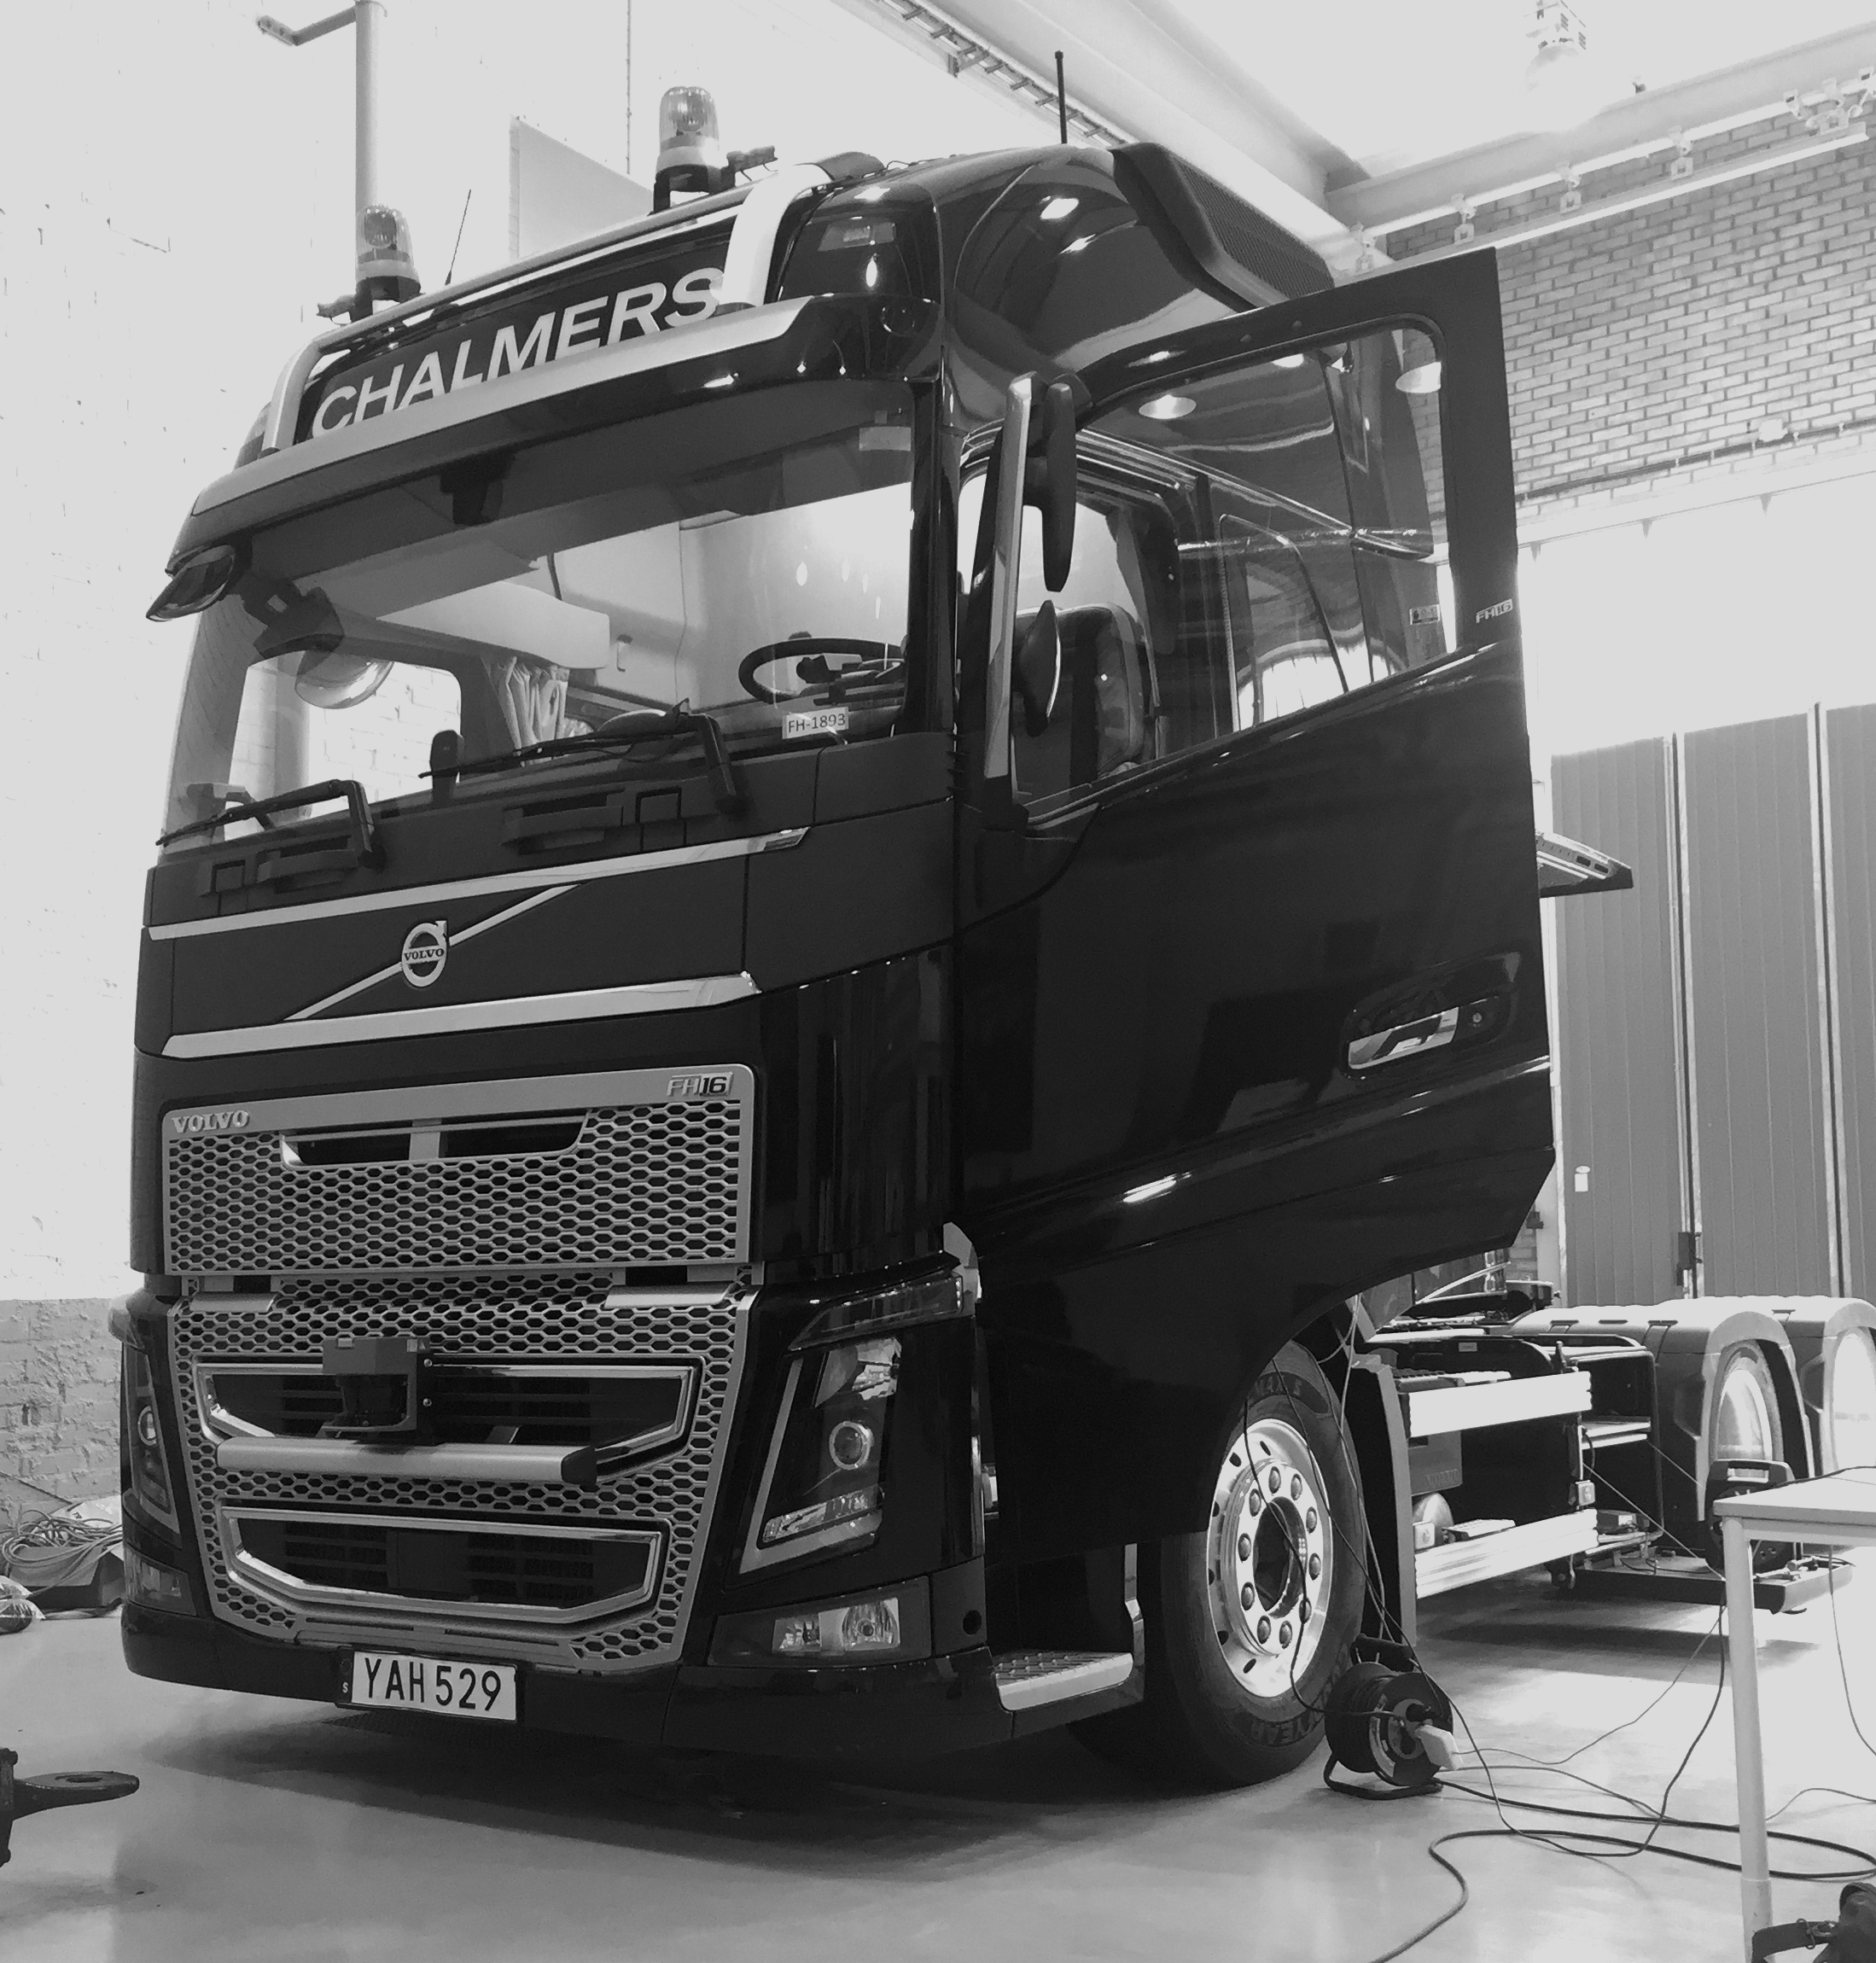
\includegraphics[width=0.5\textwidth]{./figure/truck.png}
      \caption{Chalmers Revere GCDC Truck}
       \label{truck}
\end{figure}


\section{Method}

The Pi Component from \ref{section:exp-units} is executed on a Volvo truck using precisely same hardware for the target system that is used in the experiment. The Pi component is executed on the target system natively and within a Docker container. The major difference in comparison to the experiment run is that all software components required for the Volvo truck to operate in a driver-less manner is started and run in the background: this enable a more realistic operational load but consequently a less controlled environment. Fifteen components are executed natively and within a Dockerized environment on the target system. These components are tasked with various responsibilities spanning from capturing satellite positioning data, reading data from the vehicle (e.g steering position), vehicle to vehicle communication and a number of camera operating components. Measurement points are captured via serial communication to measure the impact in a real use case. \\

The target system is running ArchLinux operating system with real-time enabled kernel, version 4.5.0-1. Docker version 1.11.1 is used for the analysis procedure and the Docker daemon is set to use the \texttt{overlayfs} storage driver, in-line with the experiment described in section \ref{soft-env}.

\section{Results}

The results shown in figure \ref{fig:truck-std-chart-noload} show that there exists a difference between the two deployment contexts in the load environment introduced by the other components running on the same system. The difference indicates that the deployment context has an impact on how deterministic a system is as native fluctuates roughly $40\%$ less than the Docker deployment context. Running a statistical test to understand the cause and effect relationship between the deployment context and the dependent variables resulted in a $\eta^{2}=0.504$ which relates to a medium effect size between deployment context and the dependent variables according to Cohen's D. Figure \ref{fig:truck-mean-chart-noload} show that there exists no average time deadline violations for either of the two execution environments.


\pgfplotstableread[col sep = semicolon]{data/truck/colsd_load.csv}\mydatanoload
\begin{figure}[H]
\caption{Std. dev. of execution environments with real-life load \textit{(lower is better)}}
\label{fig:truck-std-chart-noload}
\begin{tikzpicture}
\begin{axis}[
      xbar stacked,
      width=\textwidth*.95,
      height=\textheight*.25,
      xlabel={},
      ytick=data,
      xmin=0,
      % xmax=1.15,
      enlarge y limits={abs=1.25},
      y dir=reverse,
      xlabel={$ns$ std. dev.},
      yticklabels={Native [RT],Docker [RT]},ytick={1,...,2},
      point meta={x*100},
      legend style={
                draw=none, % ?
                text depth=0pt,
                at={(0.5,-0.25)},
                anchor=north,
                legend columns=-1,
                % default spacing:
                column sep=1cm,
                % the space between legend image and text:
                /tikz/every odd column/.append style={column sep=0cm},
            }
        ] %first axis

\addplot+[draw opacity=0,fill=orange,xbar,area legend] table[y=scenario,x=odv_oh1]{\mydatanoload};
\addplot+[draw opacity=0,fill=blues3,xbar,area legend] table[y=scenario,x=pi_calc]{\mydatanoload};
\addplot+[draw opacity=0,fill=blues5,xbar,area legend] table[y=scenario,x=odv_oh2]{\mydatanoload};
\addplot+[draw opacity=0,fill=blues1,xbar,area legend] table[y=scenario,x=sleep]{\mydatanoload};

\legend{\scriptsize Overhead 1,\scriptsize Pi calculation,\scriptsize Overhead 2,\scriptsize Sleep};
\end{axis}
\end{tikzpicture}
\end{figure}


\pgfplotstableread[col sep = semicolon]{data/truck/colsum_load.csv}\mydatanoload
\begin{figure}[H]
\caption{Execution environment mean consumed of time-slice with real-life load \textit{(closer to 1 is better)}}
\label{fig:truck-mean-chart-noload}
\begin{tikzpicture}
\begin{axis}[
        xbar stacked,
        width=\textwidth*.95,
        height=\textheight*.25,
        xlabel={},
        ytick=data,
        xmin=0,
        xmax=1.15,
        y dir=reverse,
        xlabel={$\%$ of time-slice},
        enlarge y limits={abs=1.25},
        yticklabels={Native [RT],Docker [RT]},ytick={1,...,2},
          x label style={at={(axis description cs:0.5,-0.1)},anchor=north},
        xticklabel={\scriptsize\pgfmathparse{\tick*100}\pgfmathprintnumber{\pgfmathresult}\%},
        point meta={x*100},
        legend style={
                draw=none, % ?
                text depth=0pt,
                at={(0.5,-0.22)},
                legend cell align=left,
                anchor=north,
                legend columns=3,
                % default spacing:
                column sep=1cm,
                % the space between legend image and text:
                /tikz/every odd column/.append style={column sep=0cm},
            }
        ] %first axis


\draw[black, dotted] (axis cs:1,-2) -- (axis cs:1,11);
\addplot+[draw opacity=0,fill=orange,xbar,area legend] table[y=scenario,x=odv_oh1]{\mydatanoload};
\addplot+[draw opacity=0,fill=blues3,xbar,area legend] table[y=scenario,x=pi_calc]{\mydatanoload};
\addplot+[draw opacity=0,fill=blues5,xbar,area legend] table[y=scenario,x=odv_oh2]{\mydatanoload};
\addplot+[draw opacity=0,fill=blues1,xbar,area legend] table[y=scenario,x=sleep]{\mydatanoload};

\legend{\scriptsize Overhead 1,\scriptsize Pi calculation,\scriptsize Overhead 2,\scriptsize Sleep};
\end{axis}
\end{tikzpicture}
\end{figure}
